%% using apa7 package for formatting 
%%
%% options
%%  stu  | student paper apa format
%%  12pt | font size 
%%
%% draftall if want draft water mark
\documentclass[stu, 12pt, longtable]{apa7}

%%  
%% package inserts filler text
%%
\usepackage{lipsum} 

%%
%% package formats for american english
%%
\usepackage[american]{babel}

%%
%% package that helps format in-line quotations
%%
\usepackage{csquotes}

\usepackage[author={Team 1}]{pdfcomment}


%%
%% apa style bibliography
%% sort citations by name, year, title
%% backend database is biber, default biblatex
%%
\usepackage[style=apa, sortcites=true, sorting=nyt, backend=biber]{biblatex}
\DeclareLanguageMapping{american}{american-apa}

%% adding bibliography file to list of resources
\addbibresource{bibliography.bib}


%\usepackage{caption}
%captionsetup[figure]{justification = centering, font=normal,labelfont=normal, labelformat = empty, textfont=bf}

%% all for images
% \usepackage[export]{adjustbox}
\usepackage{graphicx}
\graphicspath{ {./images/} }
% \captionsetup[figure]{justification = centering, font=normal,labelfont=normal, labelformat = empty, textfont=bf}




%% changes color of highlight 
%\usepackage[highlightmarkup=background, defaultcolor=yellow]{changes}

%% for the comments
%\usepackage{todonotes}


\title{College and Career Readiness in Charlotte, NC: An Analysis on Academic Performance, Career Readiness, and Upward Mobility.}
%% author
\authorsnames{Khem Khadka, Cody Scott, Joshua Hernandez}
%% institution

\authorsaffiliations{School of Data Science, University of North Carolina at Charlotte}
\course{DTSC 4301}
\professor{Dr.\ Tianca Crocker and Dr.\ Mary Lou Maher}
\duedate{Feburary 27, 2022 \\  \vspace{1cm} 
\includegraphics[width=8cm]{UNC_logo.png}}



%% begins the document body
\begin{document}

\maketitle

\section{Overview}
\begin{threeparttable}
    \caption{Codebook} %% the caption, required by APA7 and it looks nice :D
\label{tab:codebook} %% use this to refer to the table within the paper (I think a link will open up)
    \begin{tabular}{ p{0.17\linewidth} p{0.115\linewidth} p{0.13\linewidth} p{0.49\linewidth}}     %% 5 columns, all centered. the tabular environment begins the actual table.    
    \toprule %% A line across the top
    Variable                        & \multicolumn{3}{c}{Information} \\ %% The titles of the columns. 

                       \cmidrule(r){2-4} %% a line going across columns 2 - end
                                    &   Years    &    Type                 &  Description \\ 
\midrule
                                    &               &  Report Card        &                                    \\ 
AP\_part\_pct  & 2014-2020 &  Continuous                   &   Percent of students enrolled in AP classes\\
AP\_pass\_pct & 2014-2020 &  Continuous                   &   Percent of AP exams with a score of 3 or more     \\
enroll\_\textbf{subgroup}\tabfnm{a}& 2011-2019   &  Continuous                  &   Percent of students enrolling in college           \\
 CTE\_enroll\_pct& 2018-2020  &  Continuous                  &  Percentage of students enrolled in a CTE program     \\
CTE\_cred\_pct  & 2018-2020  &  Continuous                 &  Ratio of CTE credentials earned over students enrolled in programs          \\
\midrule
                                    &               &  NC Stats         &                     \\ 
 total\_counselors & 2015-2020  &  Discrete                  &  Guidance counselors employed district wide  \\
 int\_\textbf{intention}\tabfnm{c} & 2015-2020 &  Continuous                   &  Percent of students by post-secondary intention           \\
\midrule
&               & ISC      & \\ 
Dual Enroll                     &  ---   &     Continuous         &   Percent of students dual-enrolled\tabfnm{b}            \\
\midrule
\end{tabular}
\begin{tablenotes}[para,flushleft]
    {\small
        \textit{Note.} 

        \tabfnt{a}See table \textbf[REFERENCE TABLE OF SUBGROUPS HERE] for all subgroups.\\
        \tabfnt{b}Low-SES students, if possible.\\
        \tabfnt{c}See table \textbf[REFERENCE TABLE OF SUBGROUPS HERE] for all graduate intentions.
     }
\end{tablenotes}
\end{threeparttable}
%% American Dream Stuff

%% if want to use that graph from chetty
\begin{figure}
    \caption{Source: \cite{opportunityinsights}}
    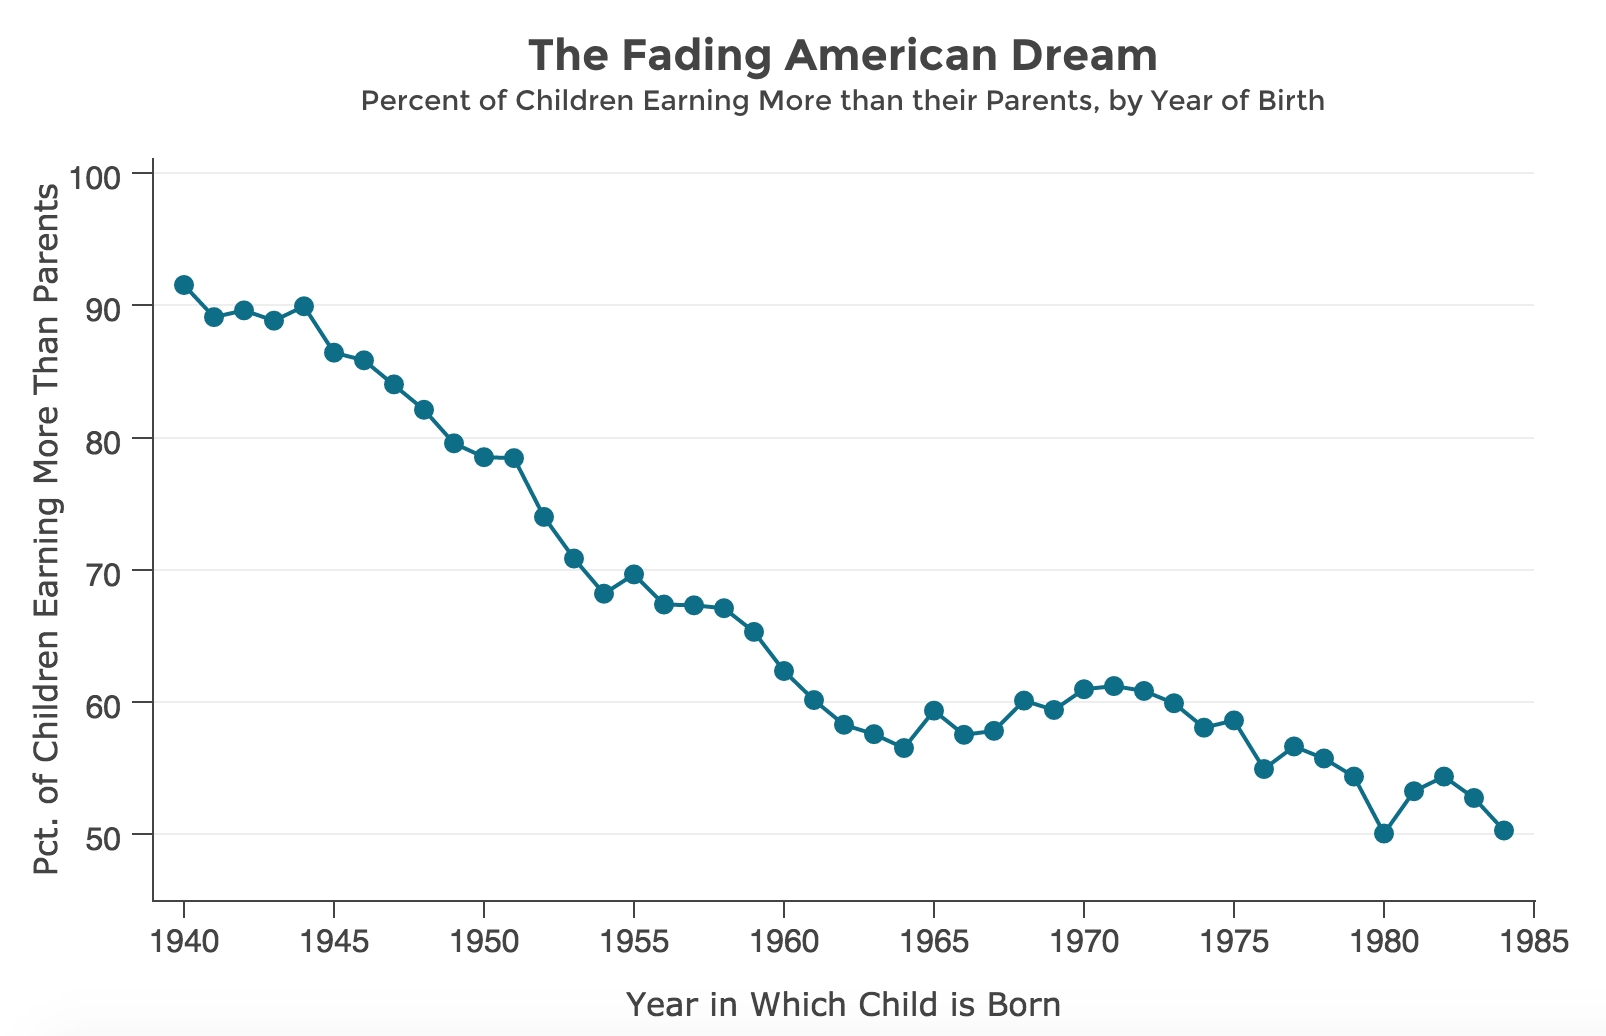
\includegraphics[width=17cm]{chetty_economic_mobility.png}
    \label{fig1}
\end{figure}





%%%%%%%%%%%%%%%%%% rest of overview

Opportunity Insights is a non-profit and partisan organization operating out of Harvard University in Massachusetts. They focus on research using large datasets to locate economic inequity. 
The team has experts in a variety of fields, using the collective disciplines to formulate solutions in battling inequality and poverty \parencite{opportunityinsights}.
Opportunity Insights is led by Director Dr. Raj Chetty, Professor of Economics at Harvard. 
As part of a broader research initiative to examine the impacts `of  tax  expenditures  on  the  budget  deficit  and  economic  activity', Chetty and his colleagues published the 2014 paper `Where is the Land of Opportunity? The Geography of Intergenerational Mobility in the United States', inspecting economic mobility of the fifty largest cities in the United States, and exploring the classic idea of the `American Dream' \parencite{opportunityinsights, chetty2014}.
Economic Mobility in this case was defined as moving from the bottom fifth income group to the top fifth group. 
They found that mobility was linked with racial and income segregation, income inequality, school quality, access to social capital, and family stability \parencite{chetty2014}.
Areas with high economic mobility were also found to have less segregation and income inequality, while having better schools, stable families, and a larger amount of social capital\parencite{chetty2014}.
Charlotte, North Carolina (NC) was included in this report, and ranked last in terms of economic mobility (Chetty et al., 2014, p. 1). Mecklenburg County was found to be 99 out of 100 counties in terms of economic mobility \parencite{opportunityinsights}. This shocked those who saw Charlotte as a growing economic hub in the South-East, but not the residents of Charlotte struggling with this economic disparity. 

In response, the city of Charlotte formed the Opportunity Task Force to address barriers of economic mobility and find solutions \parencite[][]{LOO}. The Task Force met with over 50 experts to understand the issue of intergenerational poverty, and thousands of local residents that experience this inequality first-hand \parencite[][p. ii]{LOO}. 
After 18 months of research, the Task Force published it's recommendations and formed Leading On Opportunity \parencite[][]{LOO}, a board to oversee the implementation of the recommendations in Mecklenburg County in March 2017 \parencite[][p. ii]{LOO}. 
The Task Force identified three key determinants of economic mobility and two cross-cutting factors that have an effect on all three determinants. 
Family Stability, Early Care and Education, and College and Career Readiness were the three major components to a child's ability to climb the economic ladder. Segregation (both racial and income) and Social Capital were the cross-cutting factors that can deeply affect a child's growth. 
Charlotte has a history of racial and economic segregation. 
The poor and minority neighborhoods form a `crescent' shape, while the white and rich neighborhoods are clustered in a `wedge' within the crescent \parencite[][p. iii]{LOO}. 
The home of students determines the school they go to, and in turn, the area around a school can determine the funding. It is because of this that segregation is a key issue that cannot be ignored in any three of the determinants.
\\

Likewise, social capital is associated with higher income students. Those from low-income areas may not have the resources to succeed in school that other students do \parencite[][p. viii]{LOO}. 
Safe places to study, knowledgeable and helpful mentors, and broad social networks are often not as readily available to low-socioeconomic students \parencite[][p. viii]{LOO}. 
A community that is invested in its young people and a bright future for the city is essential in increasing social capital for students \parencite[][p. iv]{LOO}. 
The Opportunity Task Force not only identified these determinants and factors, but also devised changes to be made structurally in 
Charlotte to mitigate economic barriers \parencite[][p. ii]{LOO}.
This plan included 91 recommendations, each with several implementation tactics \parencite[][p. ii]{LOO}.





\begin{figure}
    \caption{Median Household Income of Zip Code Each School Resides In}
    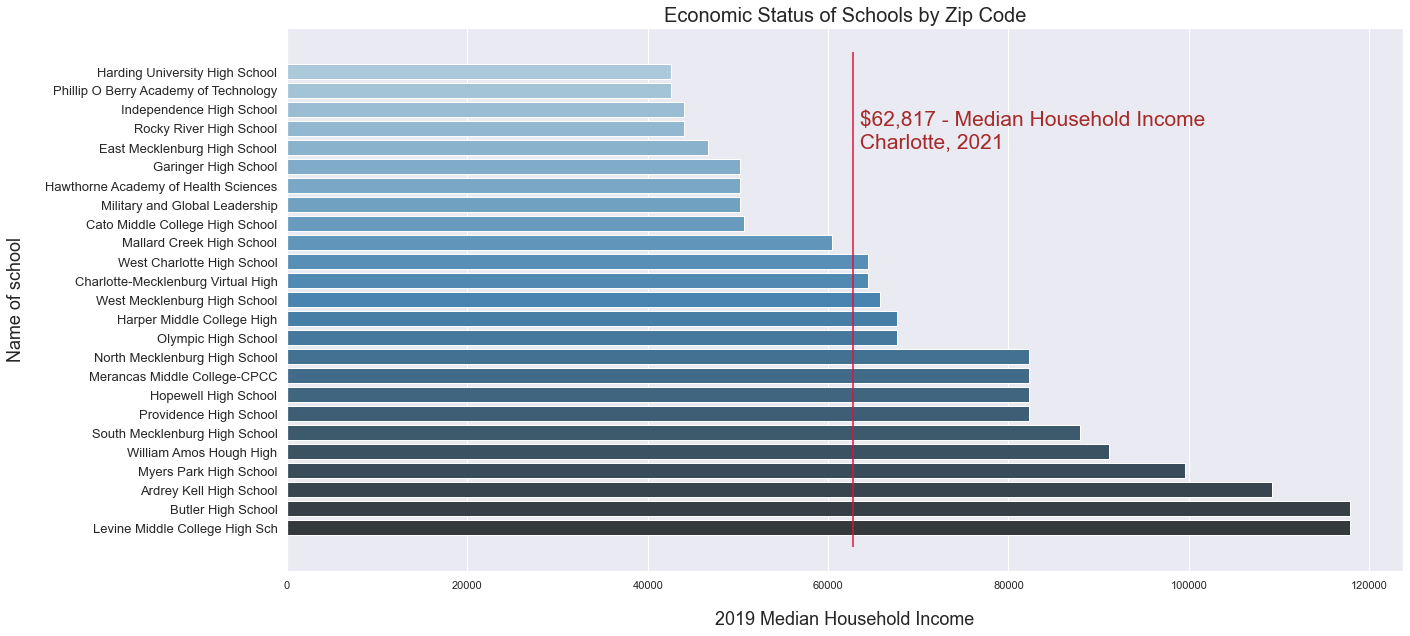
\includegraphics[width=17cm, height=10cm]{school_income.png}
    \label{fig2}
\end{figure}
Our team is focusing on Career and College Readiness in Charlotte-Mecklenburg Schools (CMS), specifically at the high school level. 

Career and College Readiness is a broad term, but generally speaks to a student's ability to enroll and succeed in college, as well as their ability to enter the workforce successfully. Charlotte-Mecklenburg Schools, much like the city itself, is a school district segregated by race and wealth. See Figure \ref{fig2} for median income by school zip code.


The demographics district wide do not represent the demographics at each school. 

\blockquote[Task Force, 2017 p. 14][]{\dots with about 39 percent, black, 29 percent white, 23 percent Latino and 6 percent Asian.\(_{9}\) A third of the 168 schools in the system are segregated by poverty, half are segregated by race and a fifth are hyper-segregated, meaning that 90 percent of their students are from a particular race.\(_{10}\) 
Over half of all African American students attend schools that are 90 percent non-white. 
The majority of white students attend majority-white schools in our high-growth southern and northern suburbs where most of our new schools have been built in recent years, as well as in more affluent close-in neighborhoods such as Myers Park and Eastover.}

With growing economic disparity, further hardships for Charlotte children should be mitigated to increase their socio-economic potential, whether that is perceived or real because of structural barriers. According to a Georgetown University study by Carnevale et al., “two of every three new jobs now require some level of postsecondary education—training credentials, an associate degree, a four-year degree, or higher” \parencite[as cited in][p. 26]{LOO}.

The actual factors that are required to guarantee a student'’'s success is unknown \parencite[][p. 27]{LOO}. 
This is why every avenue of assistance to increase a student'’'s ability to succeed should be explored. 
College can lead to future success, but technical jobs should not be written off as the requirements for those jobs evolve \parencite[][p. 27]{LOO}. 
College Readiness can be increased by more exposure to college-level studies and rigorous courses, arming students with knowledge and information ahead of their future life choices, and increasing their access to social capital. 
This can be accomplished through dual enrollment courses, such as the Career and College Promise Program, giving students access to college courses while in high school through Central Piedmont Community College (CPCC).
Guidance counselors can provide social capital to students with little or none  through their knowledge of college or career resources the students may not otherwise come into contact with \parencite{tang2019high}.
Career Readiness can involve being prepared for college, but equipping students with the knowledge and skills to succeed in the workforce out of high school is essential in preparing students for careers. 
Career and Technical Education (CTE) courses can provide students with the ability to attain relevant credentials, increasing their ability to find gainful employment immediately following graduation. Internships in the community is a way to build social capital for students while still in high school, building their network of employer contacts and recognition in the community. Also, internships can lay the foundation for full-time employment at the same company. 
Paid internships can provide supplemental means to students that would otherwise need to work at a job, freeing their time away from financial obligations by simultaneously compensating students and increasing their career-related experiences. 
By broadening the access of opportunities to more students, especially to low-socioeconomic students, Charlotte-Mecklenburg Schools can further their part in increasing the socio-economic growth of children from Mecklenburg County. 
As said best in Sprint 1, `In the end, it will not be just the high schools that need to prepare the future workforce, but it will take a partnership of primary, secondary, postsecondary, and community organizations to effectively leap the hurdle of economic mobility' \parencite[][p. 2]{sprint1}.

\section{Hypotheses}
\input{sections/Hypotheses.tex}

\section{Data Description}
An essential data source for this research is the North Carolina Department of Public Instruction (NC DPI). 
It is the organization in charge of executing educational legislation \parencite[][]{NCDPI}. NC DPI governs public, charter, and educational institutions for students with hearing and vision impairments. 
The curriculum for North Carolina (NC) is developed by the NC DPI, as it administrates accountability, finance, and administrative work throughout NC schools. 
Licensing for NC teachers is also the responsibility of the NC DPI. It oversees the data collection, in efforts to aggregate accurate school records and accountability information in an organized, accessible format \parencite[][]{NCDPI}.

The North Carolina School Report Cards is a tool utilized by the NC DPI to compile demographics, scores, and other statistics on NC schools \parencite{NCReportCards}.
Academic performance and enrollment is measured in a variety of ways, from test scores to Advanced Placement (AP) classes. 
The information ranges in years, and some features have been retired in lieu of more accurate measurements, so this data set is a bit eclectic, but comprehensive \parencite{NCReportCards}. 

Another dataset handled by the NC DPI is the North Carolina Public Schools Statistical Profile \parencite{NCStats}.
It was established in 1975 to provide open, general statistics on NC Public Schools at the state, school district, school, and charter school level \parencite{NCStats}. 
An issue that arose with this dataset was the lack of school-level data on all features. For example, data exists at the district and school level for high school graduate post secondary intentions, but not for school personnel \parencite{NCStats}. 
When following this data to the source, Common Core Data managed by the National Center for Education Statistics, it was discovered that North Carolina either did not or could not provide this granular level of data for the Common Core survey \parencite{CCD}.
Future plans to deal with this problem are addressed later in this paper. 

Charlotte's Quality of Life Explorer inspects socioeconomic and structural conditions in Mecklenburg County \parencite{quality}.
Information regarding these topics are available as interactive maps, tables, and downloadable reports by neighborhood \parencite{quality}.
Reports can be generated by filtering data geographically, allowing for unique geospatial analysis, such as the `crescent and wedge' or the light rail corridor \parencite{quality}.
This source of data was used to find the 2019 median household income by zip code in Mecklenburg County. 
This is the current placeholder value for economic data per school, and will be used to separate schools into rough economic clusters \parencite{quality}. 
\\
\begin{threeparttable}
    \caption{Codebook} %% the caption, required by APA7 and it looks nice :D
\label{tab:codebook} %% use this to refer to the table within the paper (I think a link will open up)
    \begin{tabular}{ p{0.17\linewidth} p{0.115\linewidth} p{0.13\linewidth} p{0.49\linewidth}}     %% 5 columns, all centered. the tabular environment begins the actual table.    
    \toprule %% A line across the top
    Variable                        & \multicolumn{3}{c}{Information} \\ %% The titles of the columns. 

                       \cmidrule(r){2-4} %% a line going across columns 2 - end
                                    &   Years    &    Type                 &  Description \\ 
\midrule
                                    &               &  Report Card        &                                    \\ 
AP\_part\_pct  & 2014-2020 &  Continuous                   &   Percent of students enrolled in AP classes\\
AP\_pass\_pct & 2014-2020 &  Continuous                   &   Percent of AP exams with a score of 3 or more     \\
enroll\_\textbf{subgroup}\tabfnm{a}& 2011-2019   &  Continuous                  &   Percent of students enrolling in college           \\
 CTE\_enroll\_pct& 2018-2020  &  Continuous                  &  Percentage of students enrolled in a CTE program     \\
CTE\_cred\_pct  & 2018-2020  &  Continuous                 &  Ratio of CTE credentials earned over students enrolled in programs          \\
\midrule
                                    &               &  NC Stats         &                     \\ 
 total\_counselors & 2015-2020  &  Discrete                  &  Guidance counselors employed district wide  \\
 int\_\textbf{intention}\tabfnm{c} & 2015-2020 &  Continuous                   &  Percent of students by post-secondary intention           \\
\midrule
&               & ISC      & \\ 
Dual Enroll                     &  ---   &     Continuous         &   Percent of students dual-enrolled\tabfnm{b}            \\
\midrule
\end{tabular}
\begin{tablenotes}[para,flushleft]
    {\small
        \textit{Note.} 

        \tabfnt{a}See table \textbf[REFERENCE TABLE OF SUBGROUPS HERE] for all subgroups.\\
        \tabfnt{b}Low-SES students, if possible.\\
        \tabfnt{c}See table \textbf[REFERENCE TABLE OF SUBGROUPS HERE] for all graduate intentions.
     }
\end{tablenotes}
\end{threeparttable}

\vspace{2cm}v
\begin{threeparttable}
    \renewcommand\thetable{2}
    \caption{Summary Statistics} %% the caption, required by APA7 and it looks nice :D
\label{tab:summarystats1} %% use this to refer to the table within the paper (I think a link will open up)
    \begin{tabular}{ p{0.26\linewidth} p{0.1\linewidth} p{0.1\linewidth} p{0.1\linewidth} p{0.1\linewidth} p{0.1\linewidth} p{0.1\linewidth}}     %% 5 columns, all centered. the tabular environment begins the actual table.    
    \toprule %% A line across the top
    Variable                        & \multicolumn{6}{c}{Statistics} \\ %% The titles of the columns. 

                       \cmidrule(r){2-7} %% a line going across columns 2 - end
                                    &   Non-Missing Count   &   Mean & Std & Min & Max & Missing  \\ 
\midrule 

 AP\_pass\_pct  &  195  &  0.406  & 0.23    & 0.05 & 0.87  & 42.14 \%  \\ 
 AP\_part\_pct  &  195  &  0.219  & 0.125   & 0    & 0.72  & 42.14 \%  \\ 
 int\_commcoll  &  337  &  0.35   & 0.162   & 0    & 1     & 0 \%  \\ 
 int\_pubsr     &  337  &  0.398  & 0.181   & 0    & 1     & 0 \%  \\ 
 int\_trdbusnrs &  337  &  0.016  & 0.02    & 0    & 0.139 & 0 \%  \\
 CTE\_cred\_pct &  24   &  0.143  & 0.14    & 0    & 0.54  & 92.878 \%\\
 CTE\_enroll\_pct& 78 & 0.661 & 0.148 & 0.221 & 0.98 & 76.86 \% \\
 enroll\_Disadvantaged & 209 & 0.378 & 0.219 & 0 & 0.919 & 37.982 \% \\
\midrule
\end{tabular}

\end{threeparttable}

Hypothesis 1 and 2 have both run into roadblocks in terms of operationalizing variables. In terms of operationally defined variables, the number of school counselors per high school is unavailable. 
Instead, only the district level aggregate data exists, broken down by primary and secondary schools. 
Although an increase is shown in total counselors every year, the economic disparities between Charlotte schools is not addressed with this operationalization. 
Social capital variables are the number of counselors and median household income. 
These are relatively poor proxies for social capital, considering we do not have the school level data on guidance counselors and median household income doubles as our only economic status indicator. 

Accountability laws and data collection standards are prone to change, which makes the data available change. 
CTE course enrollment and credentials earned by students was only publicly available in 2017 and on. 
This makes an analysis of Career and College Readiness before and after the formation of LOO difficult. At the same time, data that does have expanded years may be available in a retired dataset, but with different collection standards. 
For example, students participating in the College and Career Promise Program from CPCC is available from 2017 and on, however before this the data is only available for students enrolled in any postsecondary classes. 
Thus far, the hypotheses are not fully operationalized by the variables collected. 
A plan has been made to address this issue, and is covered later in this paper. 


\section{Analysis}
\subsection{Methodology}
The available data was filtered to group schools based on the median family income. 
For the year 2021, the median family income for the Charlotte region, according to the US census bureau, is \$62,817. 
As a loose grouping of schools, the schools where the median income was more than \$62,817 were classified as high socioeconomic groups and the schools where the median income was less than \$62,817 were grouped as low socioeconomic groups. 
The data was further filtered  creating datasets for before and after 2017 for each socioeconomic group. 

\subsection{Hypothesis 1}

In order to test hypothesis 1 which asserts that increasing the  numbers of mentors will eventually lead to higher college enrollment for low socioeconomic students, intention for enrolling in community college, intention for enrolling in senior institutions, AP participation rate, AP passing rate, and enrollment of disadvantaged students were considered for analysis and building model. 
Enrollment of disadvantaged students is considered as a response variable and the other variables are considered predictors. 
The correlation between the variables for both socioeconomic groups before and after  2017 were calculated. 
The correlation matrix showed that students from higher socioeconomic status, both AP participation and AP passing rate have negative correlation with intentions of enrolling in community college whereas the same variables 
have positive correlation with the intention of enrolling in senior public institutions. This indicates that the students from higher socioeconomic backgrounds who participated in AP courses are more likely to enroll in senior public institutions. 
For low socioeconomic student group, the enrollment variable and AP participation rate and AP passing rate have a higher correlation coefficient  for data after 2017. 
However, higher socioeconomic status students, AP and community college enrollment intentions are negatively or insignificantly positively correlated indicating that students from higher socioeconomic groups are less likely to intend to go to community college. 
For this group the correlation of AP with intention to enroll in senior public institutions is higher indicating that this group of students are more likely to intend to enroll in senior public institutions. 
A linear regression model was constructed using enrollment of disadvantaged as dependent variable and the rest of the variable as predictors. 
The model was tested for any multicollinearity among the predictor variables, the VIF test showed no indication of presence of multicollinearity. 
However, the parameter estimates associated with AP participation rate, AP passing rate, and community college intentions were statistically insignificant. 
Also log transformation on dependent variable indicated better linearity. 
So a final model was created, dropping the insignificant predictors and performing log transformation on the dependent variable. The model was statistically significant with improved adjusted R-square and lower standard error. 
The model passed normality and constant variance assumptions.

Correlation coefficients between the predictors and the response variable in the data before and after 2017 is shown in table \ref{tab:correlationtable}.

\begin{threeparttable}
    \caption{Correlation Coefficients} %% the caption, required by APA7 and it looks nice :D
\label{tab:correlationtable} %% use this to refer to the table within the paper (I think a link will open up)
    \begin{tabular}{>{\centering\arraybackslash} p{0.16\linewidth} p{0.2\linewidth} p{0.2\linewidth} p{0.16\linewidth} p{0.16\linewidth}}      
    \toprule %% A line across the top
    Dependent                        & \multicolumn{4}{c}{Independent} \\ %% The titles of the columns.
                        \cmidrule(r){2-5} %% a line going across columns 2 - end
                            & Intention of Community College & Intention of Public Senior Institutions & AP Participation Rate & AP Passing Rate \\ %% The titles of the columns. 
                            
\midrule
College                     &        &  \textbf{Pre 2017}   &         &         \\     
Enrollment of               &  \large0.222& \large-0.048        &  \large-0.18  & \large-0.609  \\
Economically& && &\\      \cmidrule(r){2-5}
Disadvantaged               &        &  \textbf{Post 2017}  &         &  \\
Students                    & \large0.014  &\large0.081 & \large0.1182 & \large0.112  \\
\midrule
\end{tabular}

\end{threeparttable}

The correlation coefficients among the dependent and independent variables before 2017 are all negative indicating the predictors were not positively influencing the enrollment of disadvantaged students. 
However, the correlation coefficient among the same variables after 2017 are all positive indicating that these predictors are starting to positively influence the response variable, enrollment of disadvantaged students.

The model for data after 2017 also shows no presence of multicollinearity. 
However, the summary of the model shows that none of the predictors are  significant in explaining the variability in the response variable. 
This is an issue our team is going to look into at depth in the next project. 

\subsection{Hypothesis 2}

Hypothesis 2 currently has no data on CTE enrollment and credentials earned before 2017. K-Nearest Neighbors (KNN) was discussed as a method for filling in this missing data, however, it is getting trained on only data post-2017. 
This is after the creation of LOO, which would be training data before the recommendations on data made after the recommendations. A KNN model was decided against due to this reason, as the current objective is to compare pre-2017 with post-2017 data. 
This missing data presents a problem for testing hypothesis 2. Plans for dealing with this issue are addressed later in this paper. 


\subsection{Theoretical Analysis}

% Link your findings from the analysis back to your theoretical expectations at a conceptual level, as described in your hypothesis graph. 
While constructing the hypothesis model at conceptual level, we expected that increasing the number of mentors or guidance counselors would eventually lead to higher enrollment of economically disadvantaged students. 
As the literature reviews suggested that students make better decisions when they are given the right information, and students from low socioeconomic status often lack right information for making right decision for their education choice,  we expected that increasing the number of  mentors would lead to a higher number of economically disadvantaged students choosing AP courses which would lead to higher enrollment of these students. The correlation between AP stats and enrollment of disadvantaged students was negative for data before 2017, whereas the correlation is positive for data after 2017. However, the magnitude of the relationship is small. We still  consider this as a positive sign which has the potential to make a difference in the lives of students from low socioeconomic status in the long run. For the second hypothesis our expectations have not been tested yet due to the problem of data availability. However, our group is making serious efforts to obtain relevant data from CMS and conduct the analysis. The unexpected situation created by COVID pandemic might pose a serious challenge to our effort in securing reliable data. We expect to obtain the CTE data from CMS and conduct exploration on the data to find out whether the CTE enrollment and certification has improved among the economically disadvantaged students. 

% Link Findings to theoretical expectations
%  What are the implications of your findings for how readers should think about the economic mobility problem?  


% Return back to the challenge for this project – did you address the challenge of understanding what has happened since the Task Force Report? 


% What problems or issues arose in the study that you think are important to consider?


\section{Conclusion}
The strategies and implementation tactics proposed by Opportunity Task Force appear in line with the scholarly literature. 
From increasing the number of guidance counselors to provide insight into academic and career options, to increasing the accessibility of AP courses to students from low socioeconomic backgrounds, the literature suggests that those mitigation measures in fact have shown positive effects on students \parencite[][]{castleman2014intensive}.
It is expected to see a positive correlation between the number of guidance counselors and college acceptance rates. 
Similarly, a positive relationship between counselors and the number of students obtaining CTE credentials is an expectation. 
With the implementation of a linear regression model to establish the relationship between these variables, it is anticipated to see a positive value for coefficient of the dependent variable. 
Other machine learning models are still under consideration, but the team expects to find results consistent with the hypothesis that have been presented in this paper. 
However, the details of those explorations are still underway and the team is actively looking for data that could continue to help establish those relationships. 
The next step for our team will be deciding the appropriate analysis methods and machine learning models for future prediction. 
Further research into the domain via scholarly resources is necessary to support future methods, models, and evaluation metrics that will be implemented.
The next sprint will include details of the results from the analysis and models that we will be deciding to use for making predictions, so these decisions are the topic of discussion amongst the team.


% makes the references page

\printbibliography

\appendix
\section{}
\begin{threeparttable}
    \caption{Intentions Dictionary} %% the caption, required by APA7 and it looks nice :D
\label{tab:intentions} %% use this to refer to the table within the paper (I think a link will open up)
    \begin{tabular}{ p{0.25\linewidth} p{0.3\linewidth} }     %% 5 columns, all centered. the tabular environment begins the actual table.    
    \toprule %% A line across the top
    Intention Abbreviation                        & Intention Full \\ %% The titles of the columns. 
                      % \cmidrule(r){2-4} %% a line going across columns 2 - end
\midrule
             
int\_employ                  & Employment  \\
int\_military                & Military      \\
int\_other             &       Other      \\
int\_commcoll         &   Community College    \\
int\_privjr                & Private Junior Institution     \\
int\_privsr                & Private Senior Institution     \\
int\_pubsr                &  Public Senior Institution    \\
int\_tradesch                & Trade/Business School     \\

\midrule
\end{tabular}

\end{threeparttable}
\\
\begin{threeparttable}
    \caption{Codebook} %% the caption, required by APA7 and it looks nice :D
\label{tab:codebook} %% use this to refer to the table within the paper (I think a link will open up)
    \begin{tabular}{ p{0.17\linewidth} p{0.115\linewidth} p{0.13\linewidth} p{0.49\linewidth}}     %% 5 columns, all centered. the tabular environment begins the actual table.    
    \toprule %% A line across the top
    Variable                        & \multicolumn{3}{c}{Information} \\ %% The titles of the columns. 

                       \cmidrule(r){2-4} %% a line going across columns 2 - end
                                    &   Years    &    Type                 &  Description \\ 
\midrule
                                    &               &  Report Card        &                                    \\ 
AP\_part\_pct  & 2014-2020 &  Continuous                   &   Percent of students enrolled in AP classes\\
AP\_pass\_pct & 2014-2020 &  Continuous                   &   Percent of AP exams with a score of 3 or more     \\
enroll\_\textbf{subgroup}\tabfnm{a}& 2011-2019   &  Continuous                  &   Percent of students enrolling in college           \\
 CTE\_enroll\_pct& 2018-2020  &  Continuous                  &  Percentage of students enrolled in a CTE program     \\
CTE\_cred\_pct  & 2018-2020  &  Continuous                 &  Ratio of CTE credentials earned over students enrolled in programs          \\
\midrule
                                    &               &  NC Stats         &                     \\ 
 total\_counselors & 2015-2020  &  Discrete                  &  Guidance counselors employed district wide  \\
 int\_\textbf{intention}\tabfnm{c} & 2015-2020 &  Continuous                   &  Percent of students by post-secondary intention           \\
\midrule
&               & ISC      & \\ 
Dual Enroll                     &  ---   &     Continuous         &   Percent of students dual-enrolled\tabfnm{b}            \\
\midrule
\end{tabular}
\begin{tablenotes}[para,flushleft]
    {\small
        \textit{Note.} 

        \tabfnt{a}See table \textbf[REFERENCE TABLE OF SUBGROUPS HERE] for all subgroups.\\
        \tabfnt{b}Low-SES students, if possible.\\
        \tabfnt{c}See table \textbf[REFERENCE TABLE OF SUBGROUPS HERE] for all graduate intentions.
     }
\end{tablenotes}
\end{threeparttable}
\\
\begin{threeparttable}
    \caption{Identifier Variables} %% the caption, required by APA7 and it looks nice :D
\label{tab:idvariables} %% use this to refer to the table within the paper (I think a link will open up)
    \begin{tabular}{ p{0.25\linewidth} p{0.06\linewidth} p{0.26\linewidth} p{0.34\linewidth}}     %% 5 columns, all centered. the tabular environment begins the actual table.    
    \toprule %% A line across the top
    Identifier                        & \multicolumn{3}{l}{Information} \\ %% The titles of the columns. 

                       \cmidrule(r){2-4} %% a line going across columns 2 - end
                                    &    Type   &   Use                           &  Description                                    \\ 
\midrule
                                    &            &  I.D. Variables                 &                                                 \\ 
School Name                         &    String  &  Identify school by name        & Full name of the high school                    \\
School Zip Code                     &    String  &  Assign median household income & Five-digit postal code                          \\
School Agency Code                  &    String  &  Join separate data             & Six-digit DPI code                              \\
Year                                &    String  &  Join separate data             & Year of the data                                \\
Household Median Income             &    Integer &  Identify low-income areas      & Median income of the zip code for the year 2019 \\
\midrule
\end{tabular}
\end{threeparttable}
\\
\begin{threeparttable}
    \renewcommand\thetable{2}
    \caption{Summary Statistics} %% the caption, required by APA7 and it looks nice :D
\label{tab:summarystats1} %% use this to refer to the table within the paper (I think a link will open up)
    \begin{tabular}{ p{0.26\linewidth} p{0.1\linewidth} p{0.1\linewidth} p{0.1\linewidth} p{0.1\linewidth} p{0.1\linewidth} p{0.1\linewidth}}     %% 5 columns, all centered. the tabular environment begins the actual table.    
    \toprule %% A line across the top
    Variable                        & \multicolumn{6}{c}{Statistics} \\ %% The titles of the columns. 

                       \cmidrule(r){2-7} %% a line going across columns 2 - end
                                    &   Non-Missing Count   &   Mean & Std & Min & Max & Missing  \\ 
\midrule 

 AP\_pass\_pct  &  195  &  0.406  & 0.23    & 0.05 & 0.87  & 42.14 \%  \\ 
 AP\_part\_pct  &  195  &  0.219  & 0.125   & 0    & 0.72  & 42.14 \%  \\ 
 int\_commcoll  &  337  &  0.35   & 0.162   & 0    & 1     & 0 \%  \\ 
 int\_pubsr     &  337  &  0.398  & 0.181   & 0    & 1     & 0 \%  \\ 
 int\_trdbusnrs &  337  &  0.016  & 0.02    & 0    & 0.139 & 0 \%  \\
 CTE\_cred\_pct &  24   &  0.143  & 0.14    & 0    & 0.54  & 92.878 \%\\
 CTE\_enroll\_pct& 78 & 0.661 & 0.148 & 0.221 & 0.98 & 76.86 \% \\
 enroll\_Disadvantaged & 209 & 0.378 & 0.219 & 0 & 0.919 & 37.982 \% \\
\midrule
\end{tabular}

\end{threeparttable}
\\
\begin{threeparttable}
    \caption{Summary Statistics} %% the caption, required by APA7 and it looks nice :D
\label{tab:summarystats2} %% use this to refer to the table within the paper (I think a link will open up)
    \begin{tabular}{ p{0.34\linewidth} p{0.08\linewidth} p{0.08\linewidth} p{0.08\linewidth} p{0.08\linewidth} p{0.08\linewidth} p{0.08\linewidth}}     %% 5 columns, all centered. the tabular environment begins the actual table.    
    \toprule %% A line across the top
    Variable                        & \multicolumn{6}{l}{Statistics} \\ %% The titles of the columns. 

                       \cmidrule(r){2-7} %% a line going across columns 2 - end
                                    &    Count   &   Mean & Std & Min & Max & Missing  \\ 
\midrule 
 enroll\_All &  42.0  &  0.63 & 0.17 & 0.34 & 0.95 & 0.7  \\ 
 enroll\_AmericanIndian &  0.0  &  nan & nan & nan & nan & 1.0  \\ 
 enroll\_Asian &  31.0  &  0.52 & 0.31 & 0.06 & 0.95 & 0.78  \\ 
 enroll\_Black &  88.0  &  0.41 & 0.21 & 0.06 & 0.95 & 0.38  \\ 
 enroll\_Disadvantaged &  63.0  &  0.36 & 0.19 & 0.07 & 0.85 & 0.56  \\ 
 enroll\_EnglishLearners &  12.0  &  0.3 & 0.16 & 0.05 & 0.55 & 0.92  \\ 
 enroll\_Female &  91.0  &  0.48 & 0.19 & 0.15 & 0.92 & 0.36  \\ 
 enroll\_Hispanic &  65.0  &  0.25 & 0.19 & 0.05 & 0.7 & 0.54  \\ 
 enroll\_Male &  87.0  &  0.4 & 0.18 & 0.11 & 0.84 & 0.39  \\ 
 enroll\_Twoormore &  13.0  &  0.65 & 0.21 & 0.05 & 0.93 & 0.91  \\ 
 enroll\_PacificIslander &  0.0  &  nan & nan & nan & nan & 1.0  \\ 
 enroll\_Disabilities &  16.0  &  0.39 & 0.12 & 0.24 & 0.66 & 0.89  \\ 
 enroll\_White &  63.0  &  0.52 & 0.25 & 0.05 & 0.91 & 0.56  \\ 
 CTE\_cred\_pct &  19.0  &  16.26 & 14.95 & 0.0 & 54.0 & 0.87  \\ 
 CTE\_enroll\_pct &  69.0  &  65.91 & 14.8 & 22.12 & 97.99 & 0.51  \\ 
\midrule
\end{tabular}

\end{threeparttable}


\section{}
\begin{figure}
    \caption{AP Participation Percent over Time}
    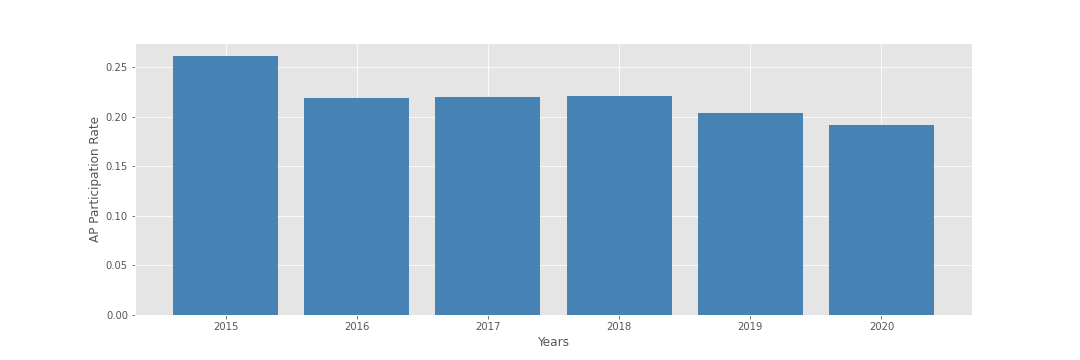
\includegraphics[width=17cm]{AP Participation Rate.png}
    \label{fig1}
\end{figure}

\begin{figure}
    \caption{AP Pass Rate over Time}
    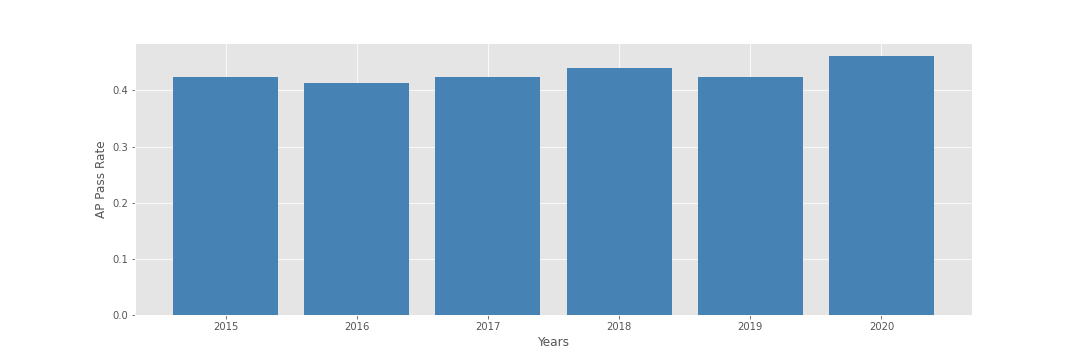
\includegraphics[width=17cm]{AP Pass Rate.png}
    \label{fig2}
\end{figure}

\begin{figure}
    \caption{CTE Student Enrollment over Time}
    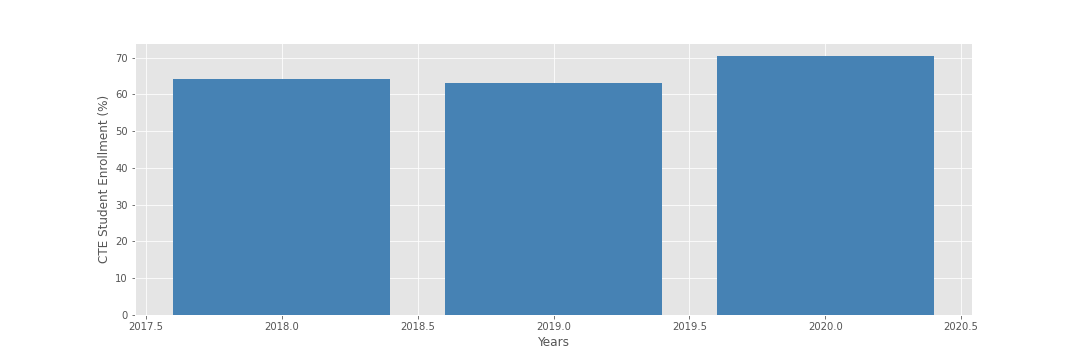
\includegraphics[width=17cm]{CTE Student Enrollment.png}
    \label{fig3}
\end{figure}

\begin{figure}
    \caption{Economically Disadvantaged Students College Enrollment over Time}
    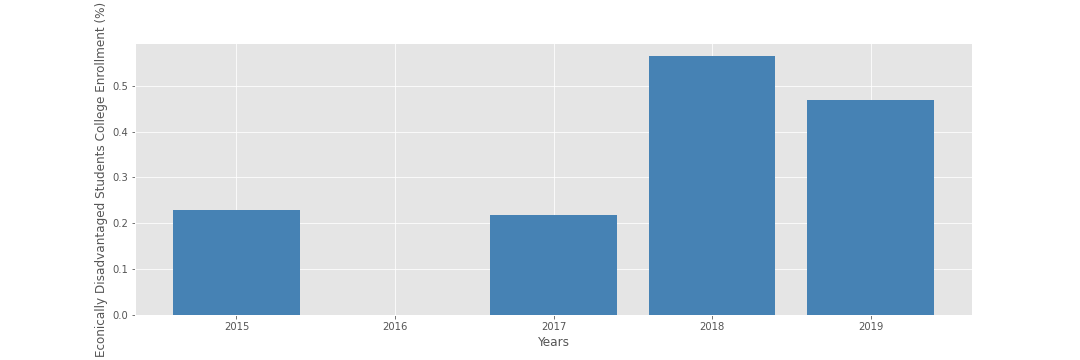
\includegraphics[width=17cm]{EDS Students College Enrollment.png}
    \label{fig4}
\end{figure}

\begin{figure}
    \caption{Number of Counselors at District Level}
    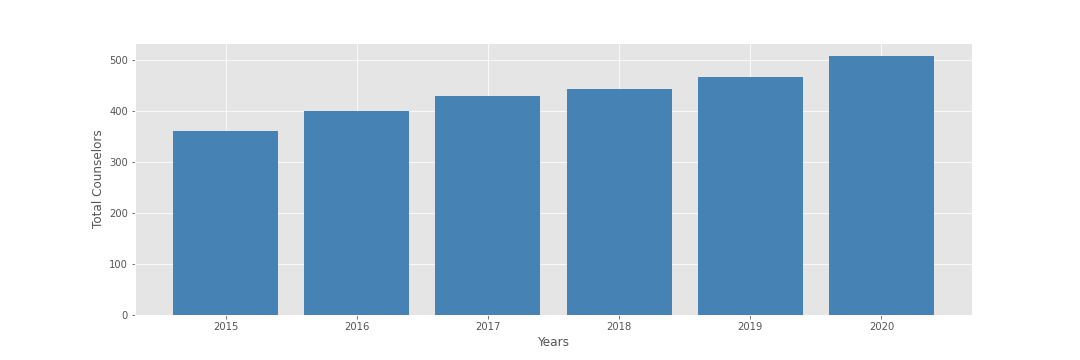
\includegraphics[width=17cm]{Total Counselors.png}
    \label{fig5}
\end{figure}



%% ends the document body
\end{document}

%% 
%% Copyright (C) 2019 by Daniel A. Weiss <daniel.weiss.led at gmail.com>
%% 
%% This work may be distributed and/or modified under the
%% conditions of the LaTeX Project Public License (LPPL), either
%% version 1.3c of this license or (at your option) any later
%% version.  The latest version of this license is in the file:
%% 
%% http://www.latex-project.org/lppl.txt
%% 
%% Users may freely modify these files without permission, as long as the
%% copyright line and this statement are maintained intact.
%% 



